%%%%%%%%%%%%%%%%%%%%%%% file template.tex %%%%%%%%%%%%%%%%%%%%%%%%%
%
% This is a template file for The European Physical Journal H
%
% Copy it to a new file with a new name and use it as the basis
% for your article
%
%%%%%%%%%%%%%%%%%%%%%%%% Springer-Verlag %%%%%%%%%%%%%%%%%%%%%%%%%%
%
\documentclass[epjH]{svjour}
%
\usepackage{graphicx,subfig,amssymb,bbm,wrapfig,listings}

%
\newcommand{\noun}[1]{\textsc{#1}}

\begin{document}
%



\title{Discrete Choice Models for Bike-Sharing Transportation Systems}
\subtitle{Supplementary Material}
\author{Juste Raimbault\inst{1}\inst{2}\fnmsep\thanks{\email{juste.raimbault@polytechnique.edu}} }
%
\institute{Graduate School, Ecole Polytechnique, Palaiseau \and LVMT, UMR-T 9403 IFSTTAR, Champs-sur-Marne}
%



\abstract{We provide here various supplementary material to the joint paper, which should ensure total reproducibility by giving technical details about processes used.\\
We detail in particular the following points :\\
\textbullet \hskip 1mm 
Discrete choice questionnaire : description of variables, implementation of the questionnaire and results of modeling.\\
\textbullet  \hskip 1mm 
Data on system dynamics : data collection process and pre-processing, descriptive statistics.\\
\textbullet  \hskip 1mm
Agent-based modeling : Model evaluation, Model implementation, Model parametrization, Model application, Gradient algorithm.
} 



%
\maketitle
%

%%%%%%%%%%%%%%%%%%%%
% 1) Discrete Choice Questionnaire
%%%%%%%%%%%%%%%%%%%%
\section{Discrete Choice Questionnaire}



%%%%%%%%%%%%%%%%%%%%
\subsection{Data structure and description}

\paragraph{Socio-economic variables\bigskip\\}

Chosen socio-economic variable are relatively simple and were designed to capture characteristics expected to be most significant. As the aim of the survey was to distinguish between modal choice that can strongly depend on ``basic\textquoteright\textquoteright profile (in the sense that using bike-sharing and bike in general has been shown to be typical behavior depending on simple types of socio-economic profiles \cite{parkin2008estimation}), this reduced choice was already accepted as providing reasonable complexity of the resulting models, especially combined with stratified choice attributes. They are the following (with respective reasons of the choice) :
\bigskip
\begin{itemize}
\item Age of people (as bike is a physical activity) ; in years.
\bigskip
\item Socio-economic category, stratified into student (1), active (2) and other (3) (as social origin but also type of occupation should influence modal choice) ; transformed into 4 boolean dummy variables (csp\_student, csp\_active, csp\_other).
\bigskip
\item If the user has a regular bike-sharing account (although this variable may not make sense directly to explain choice of bike-sharing, since the fact to register will be more a consequence of the habit to use the service than the contrary. It can be seen therefore as a control variable, useful to check internal validity of models) ; boolean variable.
\bigskip
\item Distance between residence and closest public transportation station (it is not clear if long distance but bike availability should favor bike choice, that variable was taken to check that point) ; in meters.
\bigskip
\item Weather (i.e. weather in the situation of scenarii) is also considered as a variable, as it is not alternative-dependent. Stratified with dummy variables (weather\_good, weather\_mean, weather\_hardcore).
\bigskip
\item The same way, hour of the day is considered as a variable ; in hours.
\end{itemize}

\paragraph{Attributes of scenarii\bigskip\\}

Possible modal choices are bus and bike-sharing



\paragraph{Descriptive statistics\bigskip\\}

Table 1 give basic descriptive statistics on collected data, on 288 rows of the database. Data can be directly downloaded into the biogeme format at the export address of the platform\footnote{http://37.187.242.99/Questionnaire/php/utils/export.php}. We confirm the poor quality of the data, since it is for example unbalanced in socio-economic categories.

\begin{table}
\centering
\begin{tabular}{|c|cccccc|}
  \hline
   variable & min & 1st Qrt & med & mean & 3rd Qrt & max \\
  \hline
 age & 19 & 21 & 22 & 23.95 & 24 & 50 \\
 localisation & 50 & 60 & 150 & 161.6 & 200 & 800 \\
 csp\_student & N/A & N/A & N/A & 0.75 & N/A & N/A \\
 csp\_active & N/A & N/A & N/A & 0.14 & N/A & N/A \\
 csp\_other & N/A & N/A & N/A & 0.01 & N/A & N/A \\
 subscription & N/A & N/A & N/A & 0.27 & N/A & N/A \\
 travel hour & 0 & 9 & 15 & 13.51 & 18 & 23 \\
 weather\_good & N/A & N/A & N/A & 0.44 & N/A & N/A \\
 weather\_mean & N/A & N/A & N/A & 0.35 & N/A & N/A \\
 weather\_hardcore & N/A & N/A & N/A & 0.21 & N/A & N/A \\
  \hline
\end{tabular}

\caption{Descriptive statistics of socio-economic variables. For dummies or booleans, quantile have no sense but mean gives naturally proportion of corresponding category.}

\end{table}



%%%%%%%%%%%%%%%%%%%%
\subsection{Online Questionnaire Application Architecture and implementation}

General architecture and implementation main lines were given in the paper. We provide here examples on working of the platform. Note that website is still online and source code available, for any particular concern on web architecture.

Figures 1 and 2 show the public pages available to fill the questionnaire online. These pages are the same than restricted access pages reserved to surveyors, at the exception than the latest do not need to fill security captcha at the end. Figure 3 shows the administration page, through which new questionnaire can be created (reserved to administrator). For this, total flexibility is allowed, as number of variables, attributes and choices is free, as their respective types or level in the case of attributes (one can add line by clicking on corresponding links). Once the form is filled, corresponding structures are automatically created in the SQL database, avoiding shady database administrative tasks. An capture of the database is shown in figure 4.

\begin{figure}
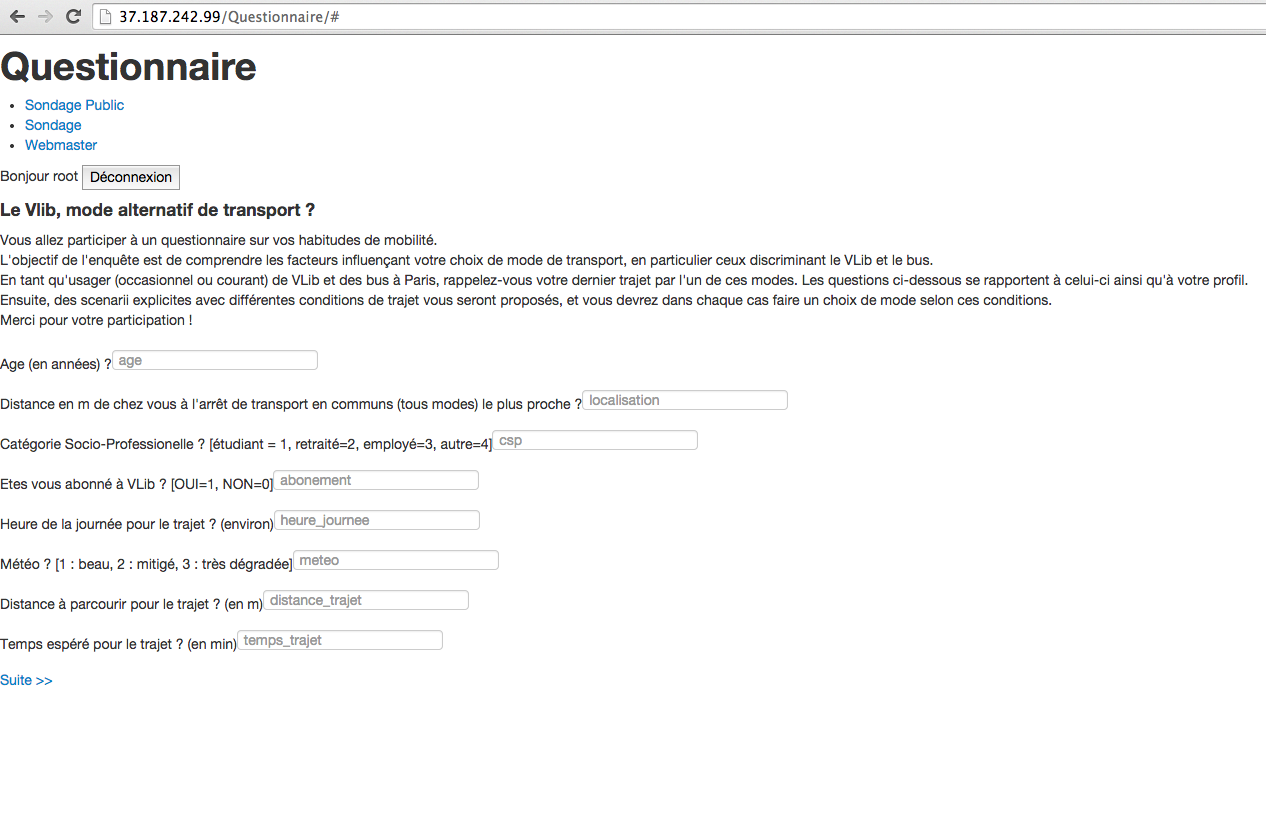
\includegraphics[angle=90,height=1.2\textheight]{figures/questionnaire}
\caption{Homepage of online questionnaire (including first part of the questionnaire).}
\label{fig:modelinterface}
\end{figure}

\begin{figure}

\includegraphics[height=\textheight]{figures/questionnaire_scenarii}
\caption{Second part of the questionnaire : scenarii and modal choices.}
\label{fig:modelinterface}
\end{figure}

\begin{figure}
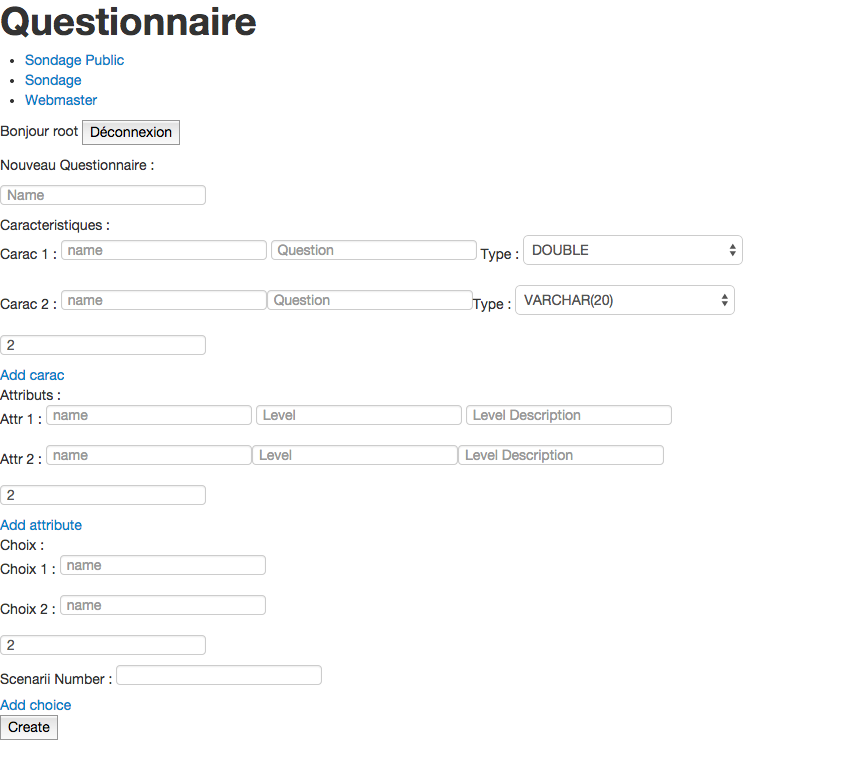
\includegraphics[height=0.8\textheight]{figures/questionnaire_webmaster}
\caption{Management page of online questionnaire.}
\label{fig:modelinterface}
\bigskip
\bigskip
\end{figure}


\begin{figure}
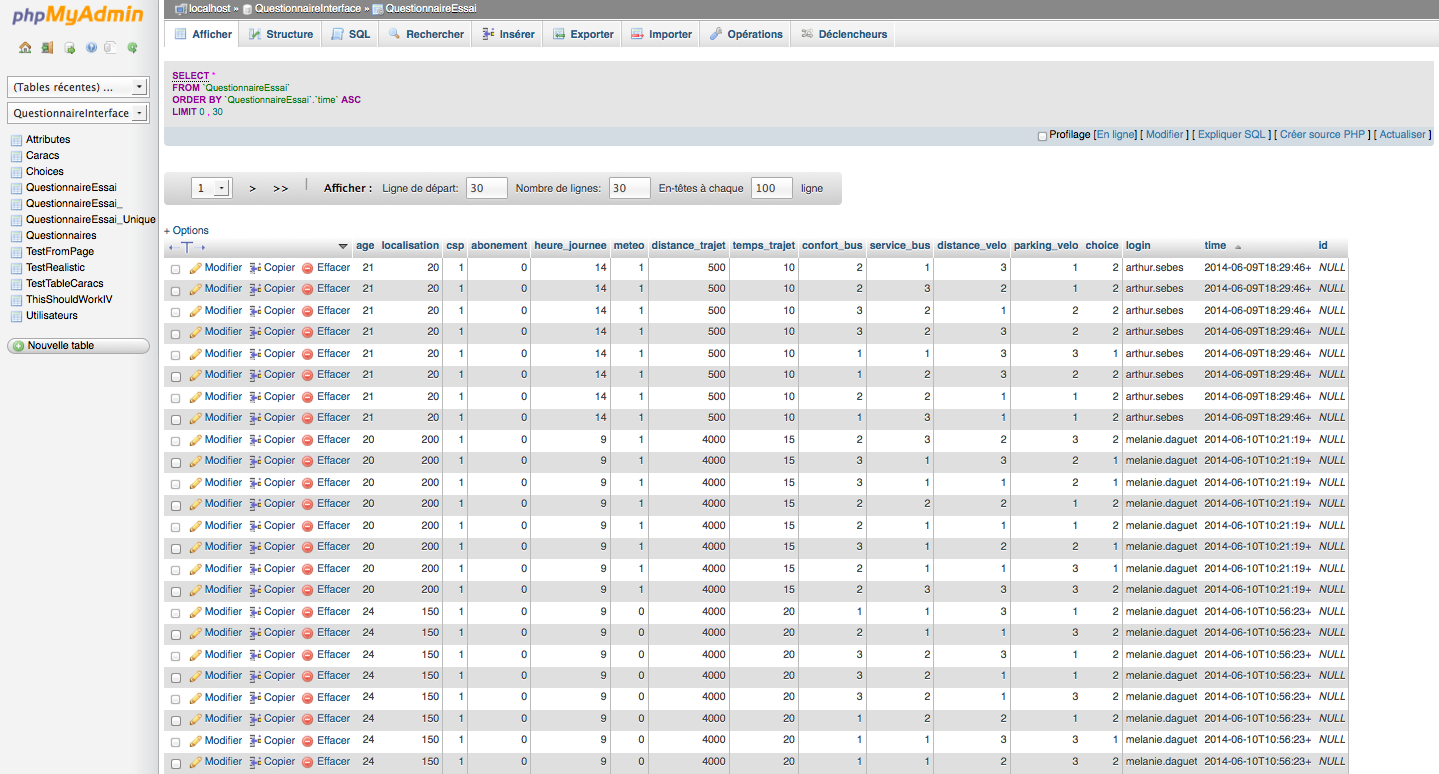
\includegraphics[angle=90,height=1.2\textheight]{figures/screenBase}
\caption{Capture of the database (through phpMyadmin mysql manager application).}
\label{fig:modelinterface}
\end{figure}


%%%%%%%%%%%%%%%%%%%%
\subsection{Modeling}

\paragraph{Full model}


%%%%%%%%%%%%%%%%%%%%
% 2) Data on system dynamics
%%%%%%%%%%%%%%%%%%%%
\section{Data on system dynamics}

%%%%%%%%%%%%%%%%%%%%
\subsection{Data Collection}

Data collection was automized, by collecting at a fixed time step during a long period of time (1 year of data used in the project, but data collection is still currently running for possible future developments of the project). Therefore, the following daemons were installed on a remote server (code is given and explained in the respective tables, as for security reasons - mainly active access ids - this code was not pushed to the git repository of the project) :
\begin{itemize}
\item  Data collection shell script. Put in crontab at a 5 minutes frequency, it collects from the operator API the real time data on stations status, provided as json data structure. See table 1 for code and explanation.
\bigskip
\item Data archiving shell script. Json file are rapidly heavy on disk (around 300Mo for one day), it is for this reason of a crucial importance to archive the data in a compressed format. Every day, a script is automatically called to archive all data file collected during the day into a single zip file, weighting 5 times less.
\end{itemize}




%% Data collection script
\begin{table}
\hrule
\begin{lstlisting}
filename=$PATHdata/`date�+``\%s``  `.json 

curl -G --data 'apiKey=`cat apiKey`&contract=Paris'
     https://api.jcdecaux.com/vls/v1/stations > $filename
\end{lstlisting}
\hrule
\medskip

\caption{Data collecting shell script.\\
Unique file identifier is created by epoch date, calling the \texttt{date} utility (echoing e.g. the number 1417980916 with the \texttt{\%s} option). Data is then collected and stored directly in file by a simple \texttt{curl} request in GET mode (\texttt{-G} option). API website returns json file of the specified contract (Paris in our case) if the user api key is valid (key is here stored in an external file and paste by \texttt{cat}.}
\label{code:datacollection}

\end{table}


%data compression
\begin{table}
\hrule
\begin{lstlisting}
#Automatic zip everyday to use 5 less memory

archivename=$PATH/archives/`date "+%s"`.zip

#need to wait for a possible current collection to be finished

p=$(ps -e | grep collect | grep -v grep)

while [ ! -z $p ]
do
  sleep 1
  p=$(ps -e | grep collect | grep -v grep)
done

#now we sure no data will be lost during zipping and removing

zip -r $archivename $PATH/data
rm -r $PATH/data
mkdir $PATH/data
\end{lstlisting}
\hrule
\medskip
\caption{Daily data archiving shell script.\\
We name the archive by the epoch date of archiving. The following loop aims to wait for any possible data collection in progress to be achieved, by listing and filtering by name the processes. We can then zip the daily data directory, remove it, and create a new empty directory for the next day.}
\label{code:dataarchiving}
\end{table}


%data remote collection
\begin{table}
\hrule
\begin{lstlisting}

#in order to deal with temporary interruption, we have a fixed local file
#with remaining zip files to download, which is updated progressively

n=$(cat remainingFiles | wc -l)

while [ $n -gt 0 ]
do
  fileName=$(head -1 remainingFiles)
  echo "Getting file "$fileName
  sshpass -p $PASSWORD scp -r $USER@$HOST:$PATH/archives/$fileName ../../Data/data
  #unzips
  echo $fileName |
      awk -F"." '{print "unzip -j -o ../../Data/data/"$1".zip -d ../../Data/data/"$1}' | sh
  #puts dir name in temp local file
  echo $fileName | awk -F"." '{print "echo "$1}' | sh >currentDir
  #calls R for file creation, that uses currentDir file and creates csv
  echo "Calling R extraction script..."
  r -f csvImport.R
  #cleaning zip and dir
  rm ../../Data/data/$fileName
  rm -R ../../Data/data/`cat currentDir`
  #putting head of files away
  tail -n `expr $n - 1` remainingFiles > tempfiles
  cat tempfiles > remainingFiles
  rm tempfiles  

  n=`expr $n - 1`

done
\end{lstlisting}
\hrule
\medskip
\caption{Remote data collection shell script.\\
This script is client-side and aims to collect and process remote raw data. File to be collected on the remote server are stored in a file (created manually for more flexibility). They are downloaded, unzipped and R script transforming heavy json into lightweight csv is called.}
\label{code:datagetremote}
\end{table}





%%%%%%%%%%%%%%%%%%%%
\subsection{Description}

A raw data file consist in a text file containing json data, more precisely an array of which each entry is a docking station, coded as a json object. An example of json record representing a docking station is :\smallskip\\

\texttt{\{"number":11029,"name":"11029 - MENILMONTANT OBERKAMPF","address":"137 BOULEVARD MENILMONTANT - 75011 PARIS",
"position":\{"lat":48.8666176586814,
"lng":2.38301344041578\},
"banking":true,"bonus":false,"status":"OPEN",\\
"contract\_name":"Paris","bike\_stands":40,
"available\_bike\_stands":12,\\
"available\_bikes":28,"last\_update":1377639873000\}}

\bigskip

Reading the record with rjson package, we construct data objects that can easily be managed. Coordinates of docking stations allow to export through rgis their position and ids in a shapefile that is then used by the agent-based model implementation. The field \texttt{bike\_stands} allows to compute the time-series of load-factors combined with \texttt{available\_bikes}. As parametrization is done on typical day extracted through the clustering procedure, we do not user the field giving status of docking station. Also, ``bonus\textquoteright\textquoteright character of a station is not taken into account in our model so we do not use that field. Furthermore, we consider for the sake of simplicity that system topology is stationary even on the larger time scale studied, i.e. we do not consider stations additions or extensions during the study period, what is a negligible approximation as less than 10 stations were extended during the period and no stations were constructed.

We show in figure 5 example of (non-normalized) load-factor curves for different docking stations, that can be dramatically different thus the need of the clustering procedure described in the main paper to isolate typical profiles and reduce dimension of the representation of the system (1230 docking stations).


\begin{figure}
\centering
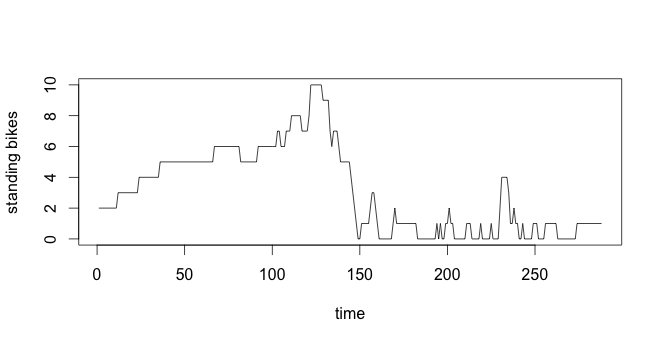
\includegraphics[trim=0cm 2cm 0cm 0cm,width=\textwidth]{figures/exTS_1.png}\\
\vspace{-0.4cm}
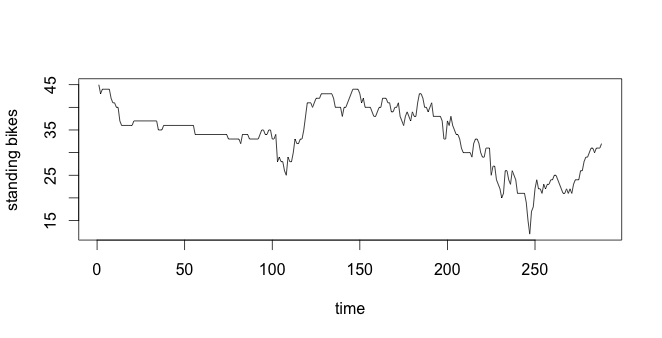
\includegraphics[trim=0cm 2cm 0cm 0cm,width=\textwidth]{figures/exTS_2.png}\\
\vspace{-0.4cm}
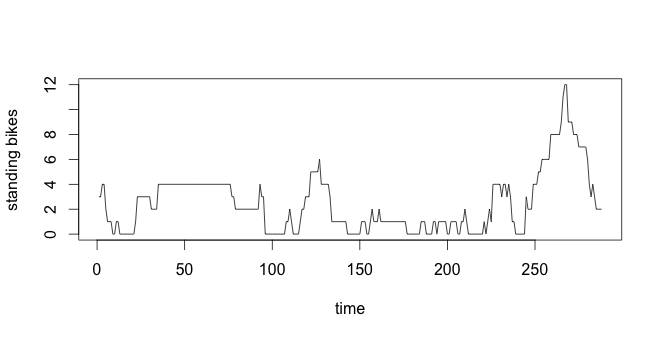
\includegraphics[trim=0cm 2cm 0cm 0cm,width=\textwidth]{figures/exTS_3.png}\\
\vspace{-0.4cm}
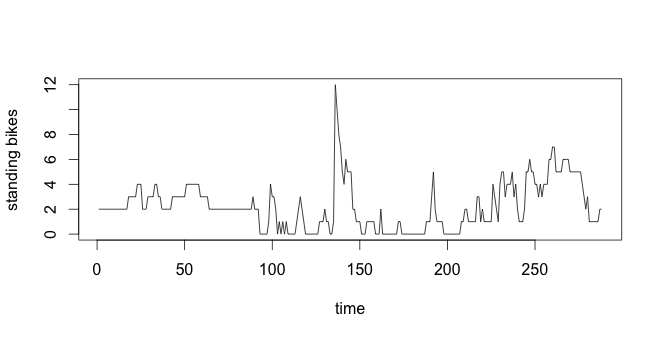
\includegraphics[trim=0cm 2cm 0cm 0cm,width=\textwidth]{figures/exTS_4.png}
\caption{Example of time-series of available bikes at different docking stations. First is a typical work area station, as number of bikes increase in the morning, to fall to quasi null in the afternoon. Second is more complicated and may be an hybrid area. The two other are zones were flux are very high, as dropped bikes directly disappear.}
\end{figure}


We show in figure 6 the geographical representation (drawn with QGIS), for which road network of Paris and neighborhood has been extracted from OpenStreetMap, and docking stations layer has been constructed from raw data. Figure 7 provides a more detailed view of data prepared to be feed into the agent-based model implementation.

\begin{figure}
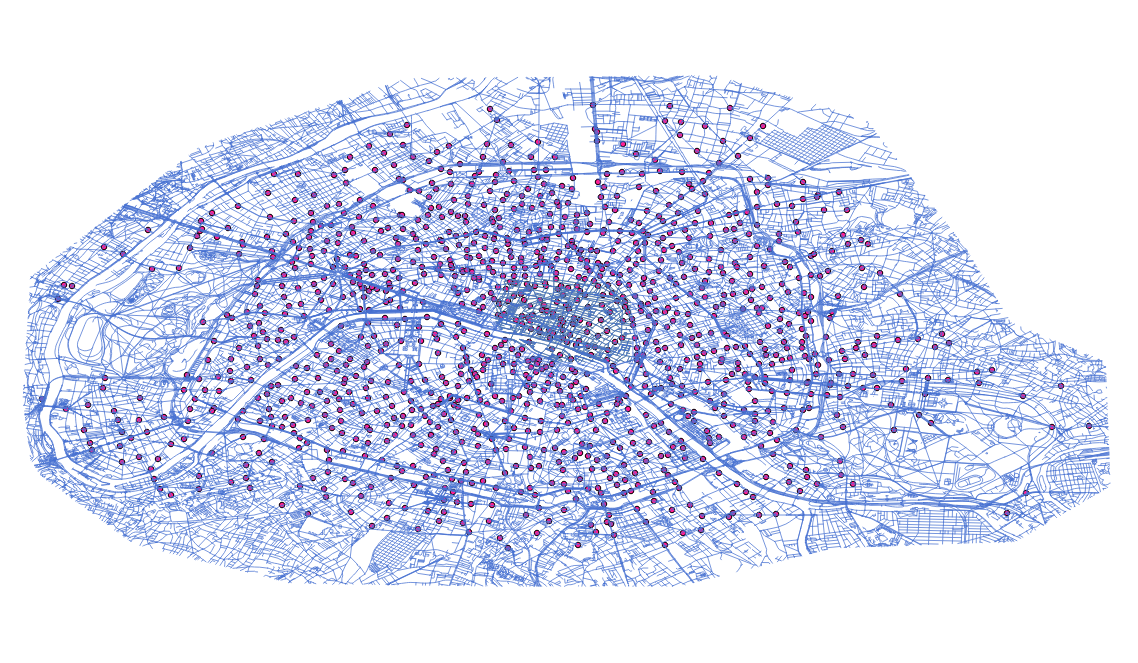
\includegraphics[angle=90,height=\textheight]{figures/gisex_paris}
\caption{Spatial representation of the system, including street network (blue) and docking stations (red).}
\end{figure}

\begin{figure}
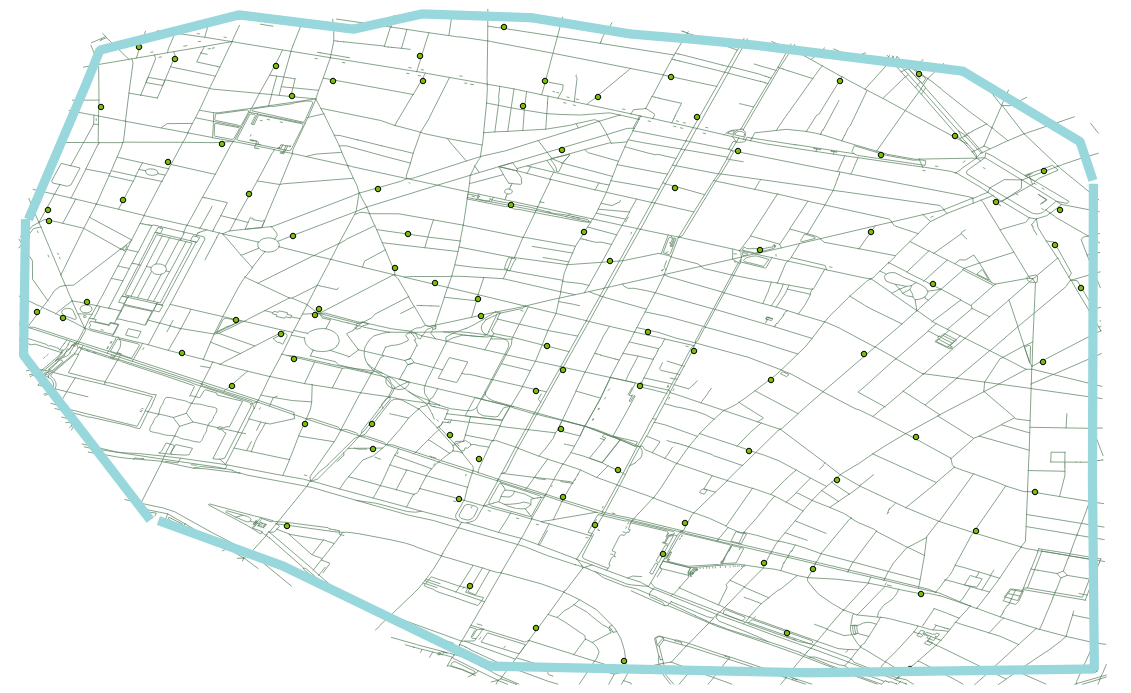
\includegraphics[width=\textwidth]{figures/gisex_district}
\caption{Construction of GIS data for a particular district. We extract the sublayer of roads (keeping all hirearchy levels in such a size of district), docking stations, and boundaries that has to be manually constructed (it is then used to determine in- and outpoints by intersecting with street network).}
\end{figure}



%%%%%%%%%%%%%%%%%%%%
% 3)  Agent-based Modeling
%%%%%%%%%%%%%%%%%%%%
\section{Agent-Based Modeling}

%%%%%%%%%%%%%%%%%%%%
\subsection{Evaluation criteria}


In order to quantify the performance of the system, to compare different realizations for different points in the parameter space or to evaluate the fitness of a realization towards real data, we need to define some functions of evaluation, proxies of what are considered as ``qualities'' of the system. Indeed, a model in itself has no use if it can not be projected in an interpretable euclidian space (in analogy to events in a probability space that take sense only through the Transfer Theorem allowing to define real probabilities).


\paragraph{Temporal evaluation functions\bigskip\\}

These are criteria evaluated at each time step and for which the output
on the all shape of the time-series will be compared.
\begin{itemize}
\item Mean load factor
\[
\bar{l}(t)=\frac{1}{\left|S\right|}\sum_{s\in S}\frac{p_{b}(s)}{c(s)}
\]

\item Heterogeneity of bike distribution: we aggregate spatial heterogeneity
of load factors on each station through a standard normalized heterogeneity
indicator, defined by
\[h(t)=\frac{2}{\sum_{s\neq s'\in S}\frac{1}{d(s,s')}}\cdot\sum_{
s\neq s'\in S}\frac{\left|\frac{p_{b}(s,t)}{c(s)}-\frac{p_{b}(s',t)}{c(s')}\right|}{d(s,s')}
\]

\end{itemize}

\paragraph{Aggregated evaluation functions\bigskip\\}

These are criteria aggregated on a all day quantifying the level of
service integrated on all travels. We note $\mathcal{T}$ the set
of travels for a realization of the system and $\mathcal{A}$ the
set of travel for which an ``adverse event'' occurred, i. e. for
which a potential dropping station was full or a starting station
was empty. For any travel $v\in\mathcal{T}$, we denote by $d_{th}(v)$
the theoretical distance (defined by the network distance between
origin and initial destination) and $d_{r}(v)$ the effective realized
distance.

\begin{itemize}

\item Proportion of adverse events: proportion of users for which the quality
of service was doubtful.
\[A=\frac{\left|\mathcal{A}\right|}{\left|\mathcal{T}\right|}\]
\item Total quantity of detours: quantification of the deviation regarding
an ideal service
\[D_{tot}=\frac{1}{\left|\mathcal{T}\right|}\cdot\sum_{v\in\mathcal{T}}\frac{d_{r}(v)}{d_{th}(v)}\]

\end{itemize}




%%%%%%%%%%%%%%%%%%%%
\subsection{Model Parametrization}

The model was designed in order to have real proxies for most of parameters. Most of parameters described in the model description section of the main paper are taken from the literature from comparable contexts and problematics.

Mean travel speed is taken as $\bar{v}=$14km.h$^{-1}$ from \cite{jensen2010characterizing}, where data of trips where studied for the bike system of the city of Lyon, France. To simplify, we take same speed for all bikers : $v(b)=\bar{v}$. A possible extension with tiny gaussian distribution around mean speed showed in experiments to bring nothing more. It has been shown in \cite{o2013mining} that profiles of use of bike systems stays approximatively the same for european cities (but can be significantly different for cities as Rio or Taipei), what justify the use of these inferred data in our case. We also use the determined mean length of travel from \cite{nair2013large} (here that parameter should be more sensible to the topology so we prefer extract it from this second paper although it seems to have subsequent methodological bias compared to the first rigorous work on the system of Lyon), which is 2.3km, in order to determine the diameter of the area on which our approach stays consistent. Indeed the model is built in order to have emphasis on travels coming from the outside and on travels going out, internal travels have to stay a small proportion of all travels. In our case, a district of diameter 2km gives a proportion of internal travels $p_{it} \approx 20\%$. We always take districts of this size with this fixed proportion in the project. 




%%%%%%%%%%%%%%%%%%%%
\subsection{Model Implementation}

\paragraph{Languages\bigskip\\}

The model was implemented in NetLogo~\cite{NetLogo} including GIS
data through the GIS extension. Preliminary treatment of GIS data
was done with the open geographic information system QGIS~\cite{QGIS_software}. Statistical pre-treatment
of real temporal data was done in R~\cite{R}, using the NL-R extension
(\cite{thiele2012agent}) to import directly the data. For complete reproducibility, source code (including data collection scripts, statistical R code and NetLogo agent-based modeling code) and data (raw and processed) are available on the open git repository of the project \footnote{at \texttt{http://github.com/JusteRaimbault/DiscreteChoiceBikeSharing}}.

\paragraph{Architecture\bigskip\\}

Following best practices typically used when developing reasonable size and complexity models with NetLogo (in the sense of more complex and complicated than a toy model but less than a fully operational data-driven model as a LUTI e.g.) we separate main model file from auxiliary source, containing agents or static procedures, in an analog way to classes in an object oriented language (being close in that sense to the GAMA language as an agent-oriented language). Model \texttt{CityBikes.nlogo} contains agent description, variables definition and includes.

We have then the following auxiliary files :
\begin{itemize}
\item Setup
\begin{itemize}
\item \texttt{setup.nls} Main setup function
\item \texttt{gis-setup.nls} GIS specific setup (layer loading and transformation into abstract agents)
\item \texttt{r-setup.nls} Import of parametrization data
\end{itemize}

\item Core
\begin{itemize}
\item \texttt{main.nls} Main runtime
\item \texttt{bikers.nls} Bikers agents
\item \texttt{depqueue.nls} Static abstract class managing walking agents
\end{itemize}

\item Evaluation : \texttt{evaluation.nls}

\item Display : \texttt{display.nls}

\item Exploration and Calibration
\begin{itemize}
\item \texttt{exploration.nls} Parameter space exploration
\item \texttt{bikers.nls} Bikers agents
\item \texttt{depqueue.nls} Static abstract class managing walking agents
\end{itemize}
\item Standard utilities

\end{itemize}




%%%%%%%%%%%%%%%%%%%%
\subsection{Model application}

We give here details on model execution and application, by first showing example of potential behaviors, then developing statistical analysis for internal validation and finally investigation on user strategies.


%% Figure interface
\begin{figure}
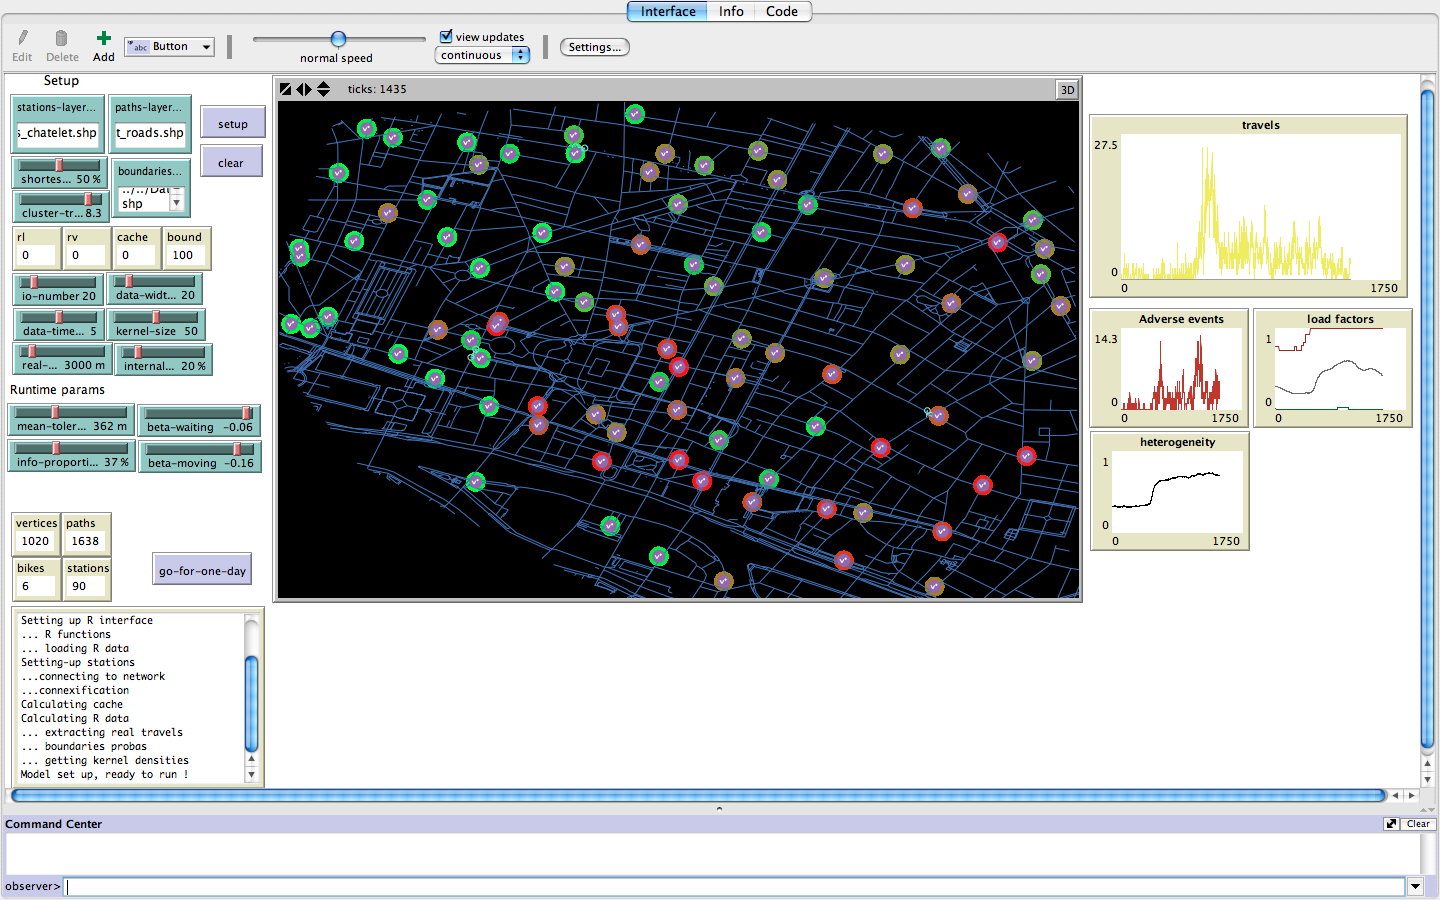
\includegraphics[angle=90,height=1.2\textheight]{figures/modelinterface}
\caption{Capture of the NetLogo model interface.}
\label{fig:modelinterface}
\end{figure}


% figure example run 1
\begin{figure}
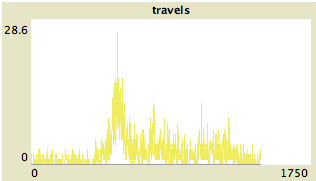
\includegraphics[width=0.57\textwidth]{figures/ex_lowpars_travels}
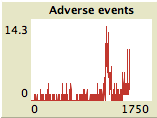
\includegraphics[width=0.43\textwidth]{figures/ex_lowpars_adverse}\\
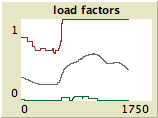
\includegraphics[width=0.5\textwidth]{figures/ex_lowpars_lf}
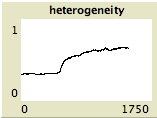
\includegraphics[width=0.5\textwidth]{figures/ex_lowpars_het}
\caption{Example of output time series for evaluation functions of the model, on a 24 hours single run. Here, tunable parameters are typically low ($p_{info}=10,r=50$) and discrete choice parameters are fixed.}
\label{fig:modelinterface}
\end{figure}

% figure example run 2
\begin{figure}
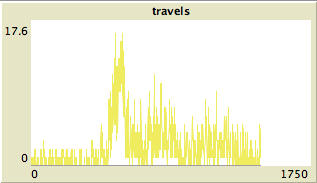
\includegraphics[width=0.57\textwidth]{figures/ex_highpars_travels}
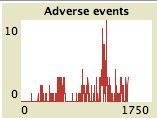
\includegraphics[width=0.43\textwidth]{figures/ex_highpars_adverse}\\
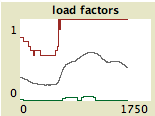
\includegraphics[width=0.5\textwidth]{figures/ex_highpars_lf}
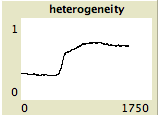
\includegraphics[width=0.5\textwidth]{figures/ex_highpars_het}
\caption{Other example of run with higher values of parameters ($p_{info}=40,r=150$). We observe differences but of small magnitude. Final heterogeneity is smaller, meaning this case is more performant in that sense. Also, more travel are done since people are more about to walk to start a travel, what means also less adverse events, what we can see on the evening period. The order of magnitude of differences confirms that the data-driven character of the model strongly governs its behavior, since patterns depend on the first order of spatial geometry and temporal evolution of parametrization time-series.}
\label{fig:modelinterface}
\end{figure}






\paragraph{Internal consistence of the model\bigskip\\}

Before using simulations of the model to explore possible strategies, it is necessary to assess that the results produced are internally consistent, i. e. that the randomness introduced in the parametrization and in the internal rules do not lead to divergences in results. Simulations were launched on a large number of repetitions for different points in the parameter space and statistical distribution of aggregated outputs were plotted. Fig. 3 shows example of these results. The relative good gaussian fits and the small deviation of distributions confirm the internal consistence of the model. We obtain the typical number of repetitions needed to have a 95\% confidence interval of length half of the standard deviation, what is around 60, and we take that number in all following experiments and applications. These experiments allowed a grid exploration of the parameter space, confirming expected behavior of indicators. In particular, the shape of $MSE$ suggested to use the simplified calibration procedure presented in the following.



%%Fig 3 : statistical analysis
\begin{figure}

\centering
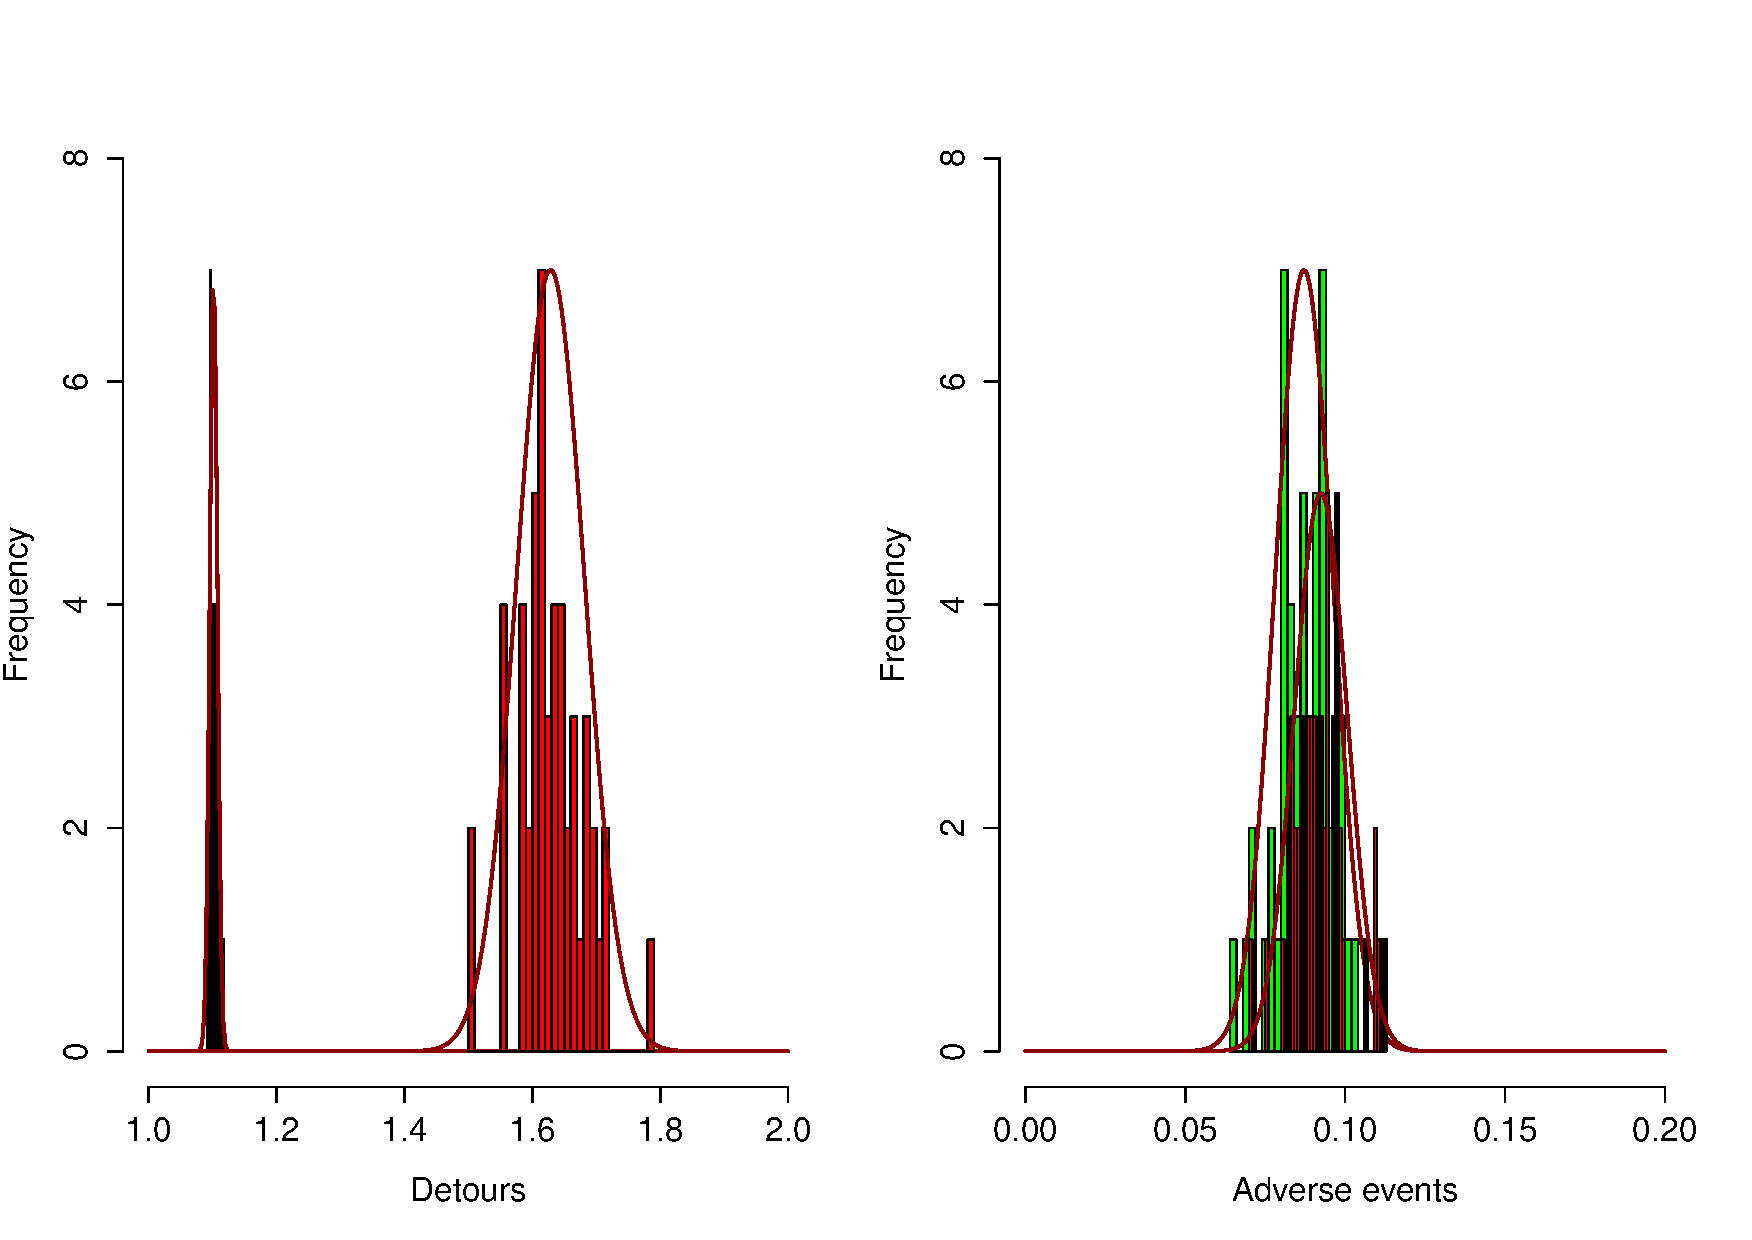
\includegraphics[width=0.9\textwidth]{figures/histogram}
\caption{Statistical analysis of outputs.\\
For some aggregated outputs (here the overall quantity of detours
and the proportion of adverse events), we plotted histograms of the
statistical distribution of the functions on many realizations of
the model for a point in the parameter space. Two points of the parameter space, corresponding to $(r=300,p_{info}=50,\sigma=80)$ (green histogram) and $(r=700,p_{info}=50,\sigma=80)$ (red) are plotted
here as examples. Gaussian fits are also drawn. The relative good fit shows
the internal consistence of the model and we are able to quantify
the typical number of repetitions needed when applying the model : supposing normal distributions for the indicator and its mean, a 95\% confidence interval of size $\sigma/2$ is obtained with  $n=(2\cdot2\sigma\!\cdot\!1.96/\sigma)^2\approx60$
}
\label{fig:3}

\end{figure}%


\paragraph{Investigation of user-based strategies\bigskip\\}


\paragraph{Influence of walking radius}

Taking for kernel-size and quantity of information the values
given by the calibration, we can test the influence of walking radius
on the performance of the system. Note that we make a strong assumption,
that is that the calibration stay valid for different values of the
radius. As we stand previously, this stays true as soon as we stay
in a reasonable range of values (we obtained 300m to 600m) for the
radius. Discrete Choice parameters stay also fixed to standard value. The influence of variations of walking radius on indicators were tested. Most interesting results are shown in figure \ref{fig:5}. Concerning the indicators evaluated on time-series ($h$ and $\bar{l}(t)$), it is hard to
have a significant conclusion since the small difference that one
can observe between curves lies inside errors bars of all curves.
For $A$, we see a decreasing of the indicator
after a certain value (300m), what is significant if we consider that
radius under that value are not realistic, since a random place in
the city should be at least in mean over 300m from a bike station. However, the results concerning the radius are not so concluding, what could be due to the presence of periodic negative feedbacks: when the mean distance between two stations is reached, repartitions concerns neighbor stations as expected, but the relation is not necessarily positive, depending on the current status of the other station. A deeper understanding and exploration of the behavior of the model regarding radius should be the object of further work. 







%%%%%%%%%%
%% Fig 5 :: walking-radius
\begin{figure}
\centering


\subfloat[{Time series of heterogeneity
indicator $h(t)$ for different values of walking radius. Small
differences between means could mislead to
a positive effect of radius on heterogeneity, but the error bars
of all curves recover themselves, what makes any conclusion non-significant.}]
{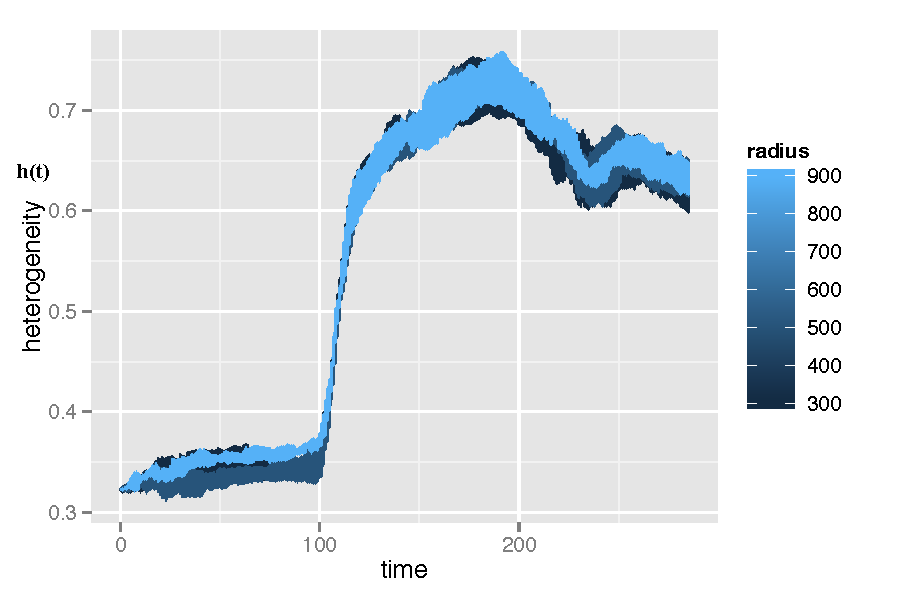
\includegraphics[trim=1cm 0.5cm 1cm 0cm,width=0.49\textwidth]{figures/hetero}}
\hfill{}
\subfloat[{Influence of walking radius
on the quantity of adverse events $A$. After 400m, we observe a relative decrease
of the proportion. However, values under 300-400m should be ignored since these
are smaller than the mean distance of a random point to a station.}]
{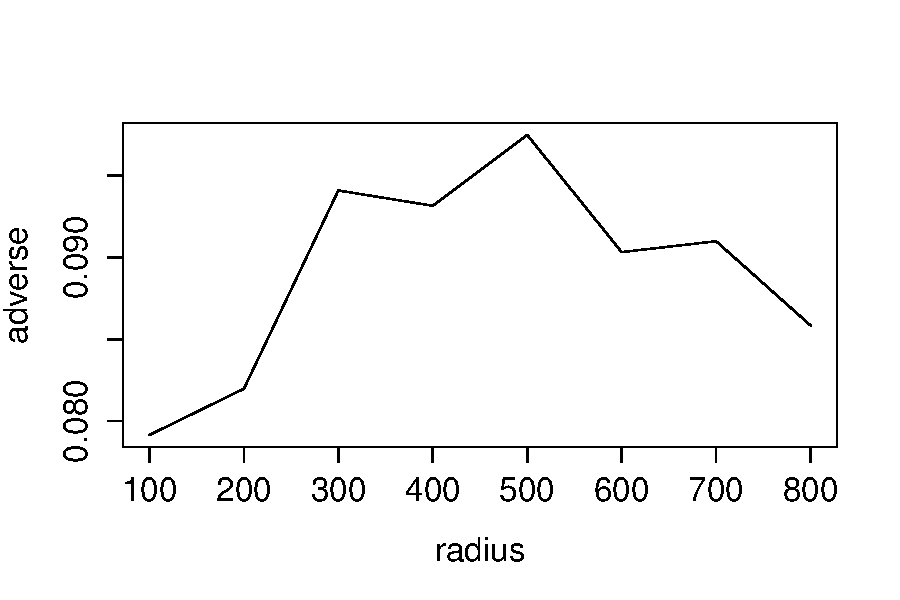
\includegraphics[trim=0cm 0.5cm 1cm 0cm,width=0.49\textwidth]{figures/adverseRadius}}

\caption{Results on the influence of walking
radius.}

%\vspace{-0.7cm}

\label{fig:5}

\end{figure}

%\vspace{-1cm}

\paragraph{Influence of information}

For the quantity of information, we are on the contrary able to draw
significant conclusions. Again, behavior of indicators were studied according to variations of $p_{info}$. Most significant are shown on figure \ref{fig6}. Results from time-series are also not concluding, but concerning aggregated indicators, we have a constant and regular
decrease for each and for different values of the radius. We are able
to quantify a critical value of the information for which most of
the progress concerning indicator $A$ (adverse events) is done, that is around 35\%.
We observe for this value an amelioration of 4\% in the quantity of
adverse events, that is interesting when compared to the total number
of bikers. Regarding the management strategy for an increase in the level of service, that implies an increase of the penetration rate of online information tools (mobile application e. g.) if that rate is below 50\%. If it is over that value, we have shown that efforts for an increase of penetration rate would be pointless.

%%%%%%% Fig 6 :: information
%%%%%%%%%%%%%%%

\begin{figure}
\centering


\subfloat[{Influence of proportion
of information on adverse events $A$ for two different values of walking
radius. We can conclude significantly that the information has a positive
influence. Quantitatively, we extract the threshold of 35\% that corresponds
to the majority of decrease, that means that more is not necessarily
needed.}]
{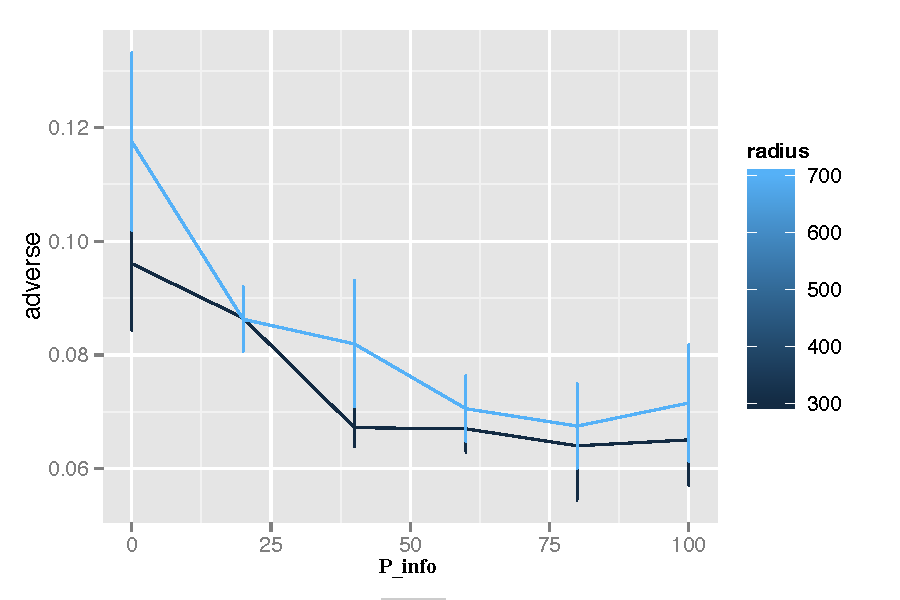
\includegraphics[trim=0cm 0cm 0cm 1cm,width=0.48\textwidth]{figures/adverse}
}\hfill{}
\subfloat[{Influence of information
on quantity of detours $D_{tot}$. Curves for $r=300m$ and $r=700m$ are shown (scale color). Here also, the influence is positive. The
effect is more significant for high values of walking radius. The inflection is around 50\% of users informed, what is more than for adverse events.}]
{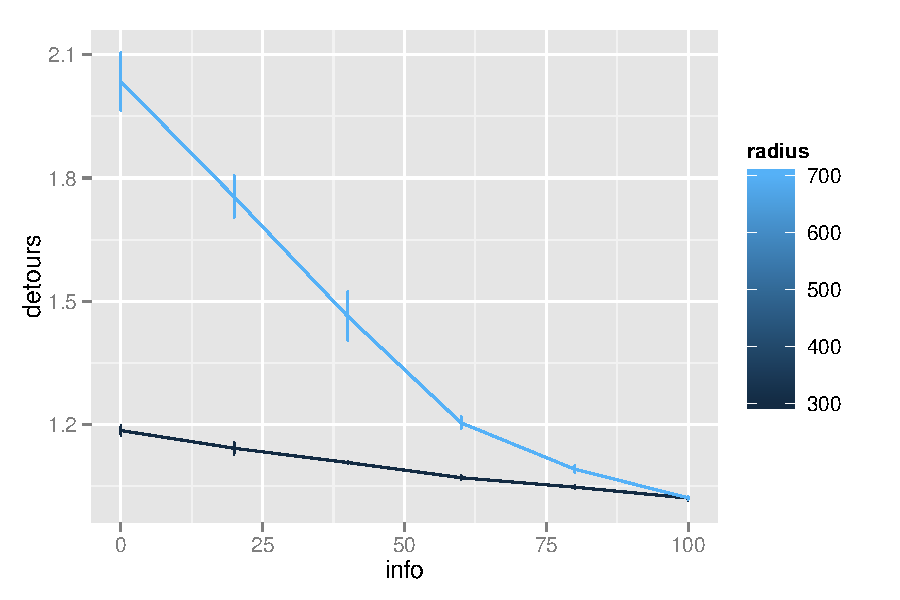
\includegraphics[trim=0cm 0cm 0cm 1cm,width=0.48\textwidth]{figures/detours}
}

\caption{Results on the influence of proportion
of information.}

%\vspace{-1.2cm}

\label{fig6}

\end{figure}
%%%%%%%%%%%%%%%%%




\subsection{Model Calibration}




\newpage


\bibliographystyle{apalike}
\bibliography{/Users/Juste/Documents/Cours/PIL/DiscreteChoicesBikeSharing/Biblio/bikesDiscreteChoices,/Users/Juste/Documents/ComplexSystems/Biblio/Bibtex/global,/Users/Juste/Documents/ComplexSystems/Biblio/Culture/Bibtex/culture,/Users/Juste/Documents/ComplexSystems/CityBikes/Biblio/bibtex,/Users/Juste/Documents/Cours/TheoreticalAnalysisComplexSystems/Project/Biblio/biblio,/Users/Juste/Documents/ComplexSystems/Misc/DynamiteSSchool2014/Biblio/dynamite}


\end{document}